\chapter{Discrete and fast Fourier transform}
\section{Discrete Fourier transform}
	The \de{Discrete Fourier Transform} (DFT) is different from the previously discussed Discrete Time Fourier Transform (DTFT); in this second case in fact the variable $\omega$, expressed in radians, is real evaluated, while in the discrete Fourier transform. Working instead with the \dft we compute a transform for a finite number of frequency samples $\omega_k \ [rad]$ with $k=0,\dots, N-1$: with this definition we can consider the DFT as a sampling of the transform in the frequency domain. In this case the discrete transform can be computed as
	\begin{equation} \label{eq:ft:dft}
		X(k) = \sum_{n=0}^{N-1} x(n) e^{-j \frac{2\pi}{N}kn} \sum_{n=0}^{N-1} x(n) W_N^{kn} \qquad \forall \ k = 0,1,\dots, N-1
	\end{equation}
	where the term $W_n^{kn}$ is referred as the \textbf{twiddle factor}.
	
	In a practical way the \dft is a sampling of the zeta transform of $N$ samples $\omega_k$ equispaced on the complex unit circle of the $\mathscr Z$ transform of the signal. Increasing the number of $N$ we decrease the \textit{distance} of $\omega_k$ and for $N\rightarrow\infty$ the DFT converges to the discrete-time Fourier transform.
	
	The \dft is not an approximated version of the DTFT, in fact for the same frequency $\omega_k$ the values are the same, but it's only a pure sampling of the continuous transform. \vspace{3mm}
	
	The \dft, in this sense, allow to estimate automatically (that can in fact be computed by machines) the transform of generic non deterministic signals. In practise we don't use the \dft but the \de{Fast Fourier Transform}, a class of complementary algorithms that allows to compute the transform in a faster way (respect to the DFT definition). \vspace{3mm}
	
	Considering the equation \ref{eq:ft:dft} we can see that this expression maxes sense only for signal with a finite number of sample (points); in particular to correctly compute the \dft the number of samples for the sequence $x(n)$ is truncated to $N$ (and having less samples than the decided resolution for $N$, we have to decrease the number of sampling in the transform). The number of frequency samples has to be equal or greater to the number of signal samples.
	
	\paragraph{Inverse Discrete Fourier Transform} In order to compute instead the \de{Inverse Discrete Fourier Transform} (IDFT) we can use the following definition:
	\begin{equation} \label{eq:ft:idft}
		x(n) = \frac 1 N \sum_{k=0}^{N-1} X(k) e^{j\frac{2\pi}{N} kn} \qquad \forall \ n = 0,1,\dots,N-1
	\end{equation}
	This is indeed the inversion of the linear problem of the equation \ref{eq:ft:dft} considering that there are $N$ equations ($X(i)$ for $i=0,\dots, N-1$) having $N$ samples each. Considering that the coefficients are $W_N^{kn}$ we can define the vectorial form of equation \ref{eq:ft:dft} as $\boldsymbol X = W \boldsymbol x$ and so $\boldsymbol x = W^{-1} \boldsymbol X$ (where $K \in \mathds R^{N\times N}$ is the coefficient matrix that's for sure non singular).
	
\subsection{Time aliasing problem}
	Given an arbitrary sequence $x(n)$ whose discrete time Fourier transform is expressed as $X(e^{j\omega})$. By computing the inverse discrete time Fourier transform we can simply reconstruct the original signal, however if we consider the \dft  $X(k)$ of the signal and we invert the result we see that the reconstructed signal $\tilde x(n)$ that's equal to the original signal only for a finite number of samples, and in particular $\tilde x(n) = x(n)$ only for $n=0,1,\dots, N-1$ and only if $N$ is longer then the input sequence length.
	
	Applying the definition of inverse \dft (eq. \ref{eq:ft:idft}) we can see that the reconstructed signal $\tilde x(n)$ must be necessarily a periodic function in time (due  to the linear combination of the twiddle factors) and so
	\[ \tilde x(n) = \frac 1 N \sum_{k=0}^{N-1} X(k) e^{j\frac{2\pi}{N} kn} = \sum_{r=-\infty}^\infty x(n-rN) \]
	
	Given $L$ the number of non-zero samples of the original signal $x(n)$ and compute a \dft with $N$ samples; if $N<L$ then we have the time aliasing problem, while we don't see this problem for $N\geq L$. The number of overlapping samples is equal to $L-N$. If we want only to perform a spectrum analyses (that wont' be followed by a reconstruction) this relations are not necessary (and we can choose any value of $N$).
	
	\begin{SCfigure}[2][bht]
		\centering 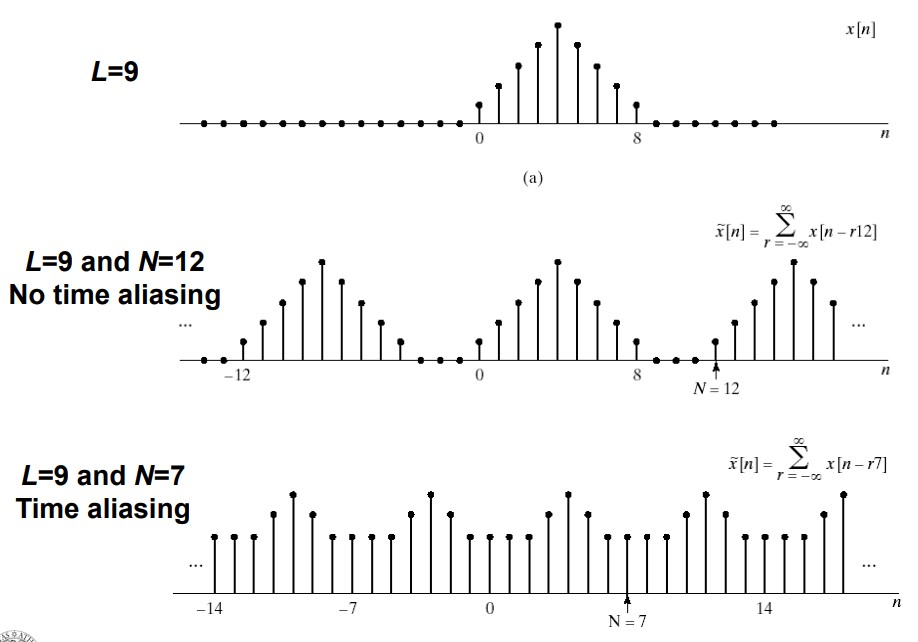
\includegraphics[width=8.5cm]{time-aliasing}
		\caption{original sequence $x(n)$ (on top) with $L=9$ and reconstructed signals $\tilde x(n)$ changing $N$ to $12 (>L)$ and $7 (<L)$. }
	\end{SCfigure}
	
	This concept is the dual result of the spectral replicas that are present in the sampling process on the time domain (in this case we are sampling in the frequency domain and so we have aliasing replicas in time domain).

\subsection{Properties}
	The \dft is a \textbf{linear operator}, in fact given two sequences $x_1(n),x_2(n)$ having discrete transforms $X_1(k),X_2(k)$ then
	\[ a x_1(n) + b x_2(n) \quad \mapsto \quad a X_1(k) + bX_2(k) \qquad \forall a,b \in \mathds R \]
	In particular if the two sequences have different length (for example $N_1 < N_2$) a number of $|N_2-N_1|$ should be added to the shorter sequence, so by doing a \textbf{zero padding}.
	
	We can also consider the \textbf{circular shifting} property that given a sequence $x(n)$ of $N$ samples with \dft $X(k)$, then given a time shift of $m\in \mathds Z$ samples in time determines a sequence
	\[ \tilde x(n-m) \ n = 0,\dots, N-1\quad \mapsto \quad X(k) e^{-j \frac{2\pi k}{N}m} \]
	where $\tilde x(n)$ is the \textit{infinite repetition} of the signal $x(n)$ (concatenation of the same signal). If the original signal $x(n)$ is real evaluated, then $\Re \{ X(k) \} = \Re \{ X(N-k) \}$ (even symmetry on the real axis) and $\Im \{X(k)\} = - \Im \{X(N-k)\}$. 

	Another property is the \textbf{circular convolution} and so given two signals $x_1,x_2 \mapsto X_1,X_2$, then
	\begin{equation}
		x_3(n):=x_1(n) * x_2(n) \mapsto X_1(k)X_2(k)  = X_3(k) \qquad k = 0,\dots, N-1
	\end{equation}
	By computing now the inverse \dft (with $N$ samples) on this result the result that we get is not the original signal $x_3(n)$, but $\tilde x_3(n)$ that's equal to $\tilde x_1(n) * x_2(n) = x_1(n) * \tilde x_2(n)$ (and this is due to the periodicity of the signals). Considering that this convolution is performed over $N$ samples, this operation is now called \textbf{circular convolution} $x_1(n) \circconv{N} x_2(n)$ defined as
	\begin{equation}
		x_1(n) \circconv{N} x_2(n) : = \sum_{m=0}^{N-1} x_1(m) \tilde x_2(n-m)
	\end{equation}
	Considering that $x_1$ consists of $L$ values, while $x_2$ consist of $P$ point, than if the \dft sampling point is equal to $N \geq L + P - 1$ then $x_1(n) * x_2(n) = x_1(n) \circconv N x_2(n)$, otherwise the result of the linear convolution and the circular one can be different.
	
	\paragraph{Impulse response} As described at page \pageref{sec:impulseresponse}, we denote as $h(n)$ the impulse response of a system and in case of a finite impulse response (FIR) one we have that $h(n) \neq 0$ for $n=0,\dots,P-1$. Assuming to have an input sequence $x(n)$ fed into the system will determine an output sequence $y(n)$ that's equal to
	\[ y(n) = x(n) * h(n) \] 
	
	Considering that also the input $x(n)$ as a finite number $L$ of samples, then the length of the convolution $y(n)$ will be different from zero for $n=0,\dots, L+P-2$ (and so it present $L+P-1$ samples). In general a way to solve this kind of problem can be solved in the frequency domain. Considering the discrete time Fourier (DTFT) transform $\F$, known the transforms $H(e^{j\omega}), X(e^{j\omega})$ of the system impulse response and input sequence, than the output can be computed as
	\[ Y(e^{j\omega}) = H(e^{j\omega}) X(e^{j\omega}) \qquad \xrightarrow{\mathscr{F}^{-1}} \quad y(n) \]
	In general this operation using the \dft (DFT), that's practically what happens, is more complex. Given the two discrete transform $X(k),H(k)$ of both the input and the impulse response, we can compute the output frequency response $Y(k) = H(k) X(k)$ that can be inverted to $y(n)$. In order to do perform this operation correctly (and not losing information due to time aliasing) the two transform have to be computed doing a zero padding for $x(n)$ with $P-1$ zero and a padding of $L-1$ zero for $h(n)$: in this case we are sure that the product $X(n)H(n)$ has a number of samples $N = L+P$ that's greater than the $L+P-1$ due to the convolution.

\section{Fast Fourier transform}
	The \de{\fft}, as already stated, is not the same as the \dft but represent a class of algorithms that are implemented to compute the Fourier transform in a \textit{faster} way (by doing less mathematical computation than the original statement).
	
	Starting from the definition on page \pageref{eq:ft:dft} of the \dft we can see that to determine the spectrum we need to perform $N-1$ complex addition and $N$ complex multiplications for each spectral sample, and so the full number of operation to perform is
	\[ N(N-1) \textrm{ complex addition} \quad + \quad N^2 \textrm{ complex multiplication} \]
	Considering that computers can't handle complex number but only real values, it means that one complex multiplication corresponds to 4 multiplications and 2 additions in the real domain (and one complex addition corresponds to 2 real additions). We can see that in general the order of complexity of the \dft is equal to
	\[ \mathcal O \big(N^2\big)\]
	
	The \fft allow to reduce the order of complexity of the operation op to the value $\mathcal O \big(N \log_2 N\big)$ (that's the ideal target value for all the algorithms) then $N$ is a power of 2, and so can be rewritten as $N = 2^\nu$ with $\nu \in \mathds N$. When this conditions is not met, usually the input sampled signal is subdivided in sequences that met the condition, perform the FFT and then recombine the result.
	
\subsection{Decimation in time FFT}
	The basic idea of the \de{decimation in time} DIT \fft algorithm is to recursively decompose the original DFT into more transforms with smaller number of points obtained through bisection.
	
	Considering for example the sequence $x(n) \neq 0$ for $n=0,\dots, N_1$ with $N = 2^\nu$, we can compute two subsequence determined by the sample in even $x_e$ and odd $x_o$ positions, having $N/2$ samples each:
	\[ \underbrace{x(0),x(2),\dots,x(N-2)}_{x_e(n) = x(2r)} \qquad \underbrace{x(1), x(3),\dots, x(N-1)}_{x_o(n) = x(2r + 1)}  \]
	
	Based on the definition (eq. \ref{eq:ft:dft}) of the \dft, we can compute the transform as
	\[ X(k) = \sum_{n=0}^{N-1} x(n) W_N^{kn} = \sum_{r=0}^{\frac N 2 - 1 } x(2r) W_N^{2rk} + \sum_{r=0}^{\frac N 2 - 1} x(2r+1) W_N^{(2r+1)k} \]
	where $W_N = e^{-j\frac{2\pi}{N}}$ is the twiddle factor. We can see that $W_N^2 = W_{N/2}$, in fact
	\[ W_N^2 = e^{-j\frac{2\pi}{N} 2 } = e^{-j\frac{2\pi}{N/2} } = W_{N/2} \]
	and so the previous expression can be rewritten as
	\[ \begin{aligned}
		X(k) & =  \sum_{r=0}^{\frac N 2 - 1 } x_e(r) W_{N/2}^{rk} + W_{N}^k  \sum_{r=0}^{\frac N 2 - 1 } x_o(r) W_{N/2}^{rk} \\ & = X_e(n) + W_N^k X_o(k)  
	\end{aligned} \qquad \qquad \qquad k = 0,\dots,N-1\]
	We can now see that the first sum corresponds to the \dft of the original signal computed only on the even position of $x(t)$, while the second sum corresponds to the odd elements. We can see that computing the transforms $X_e(k),X_o(k)$ requires a number of operation proportional to $(N/2)^2 = N^2/4$, requiring so $1/4$ of the original operations to perform the \textit{pure} transform $X(k)$. If we neglect the time computation of performing the addiction of $X_e+X_o$, than the overall number of operation is
	\[ X_e(k) + X_o(k) \propto \frac{N^2}{4} + \frac{N^2}{4} + N = \frac{N^2}{2} + N \leq N^2 \]
	where the last inequality is always verified for $N>2$.
	\begin{SCfigure}[2][bht]
		\centering 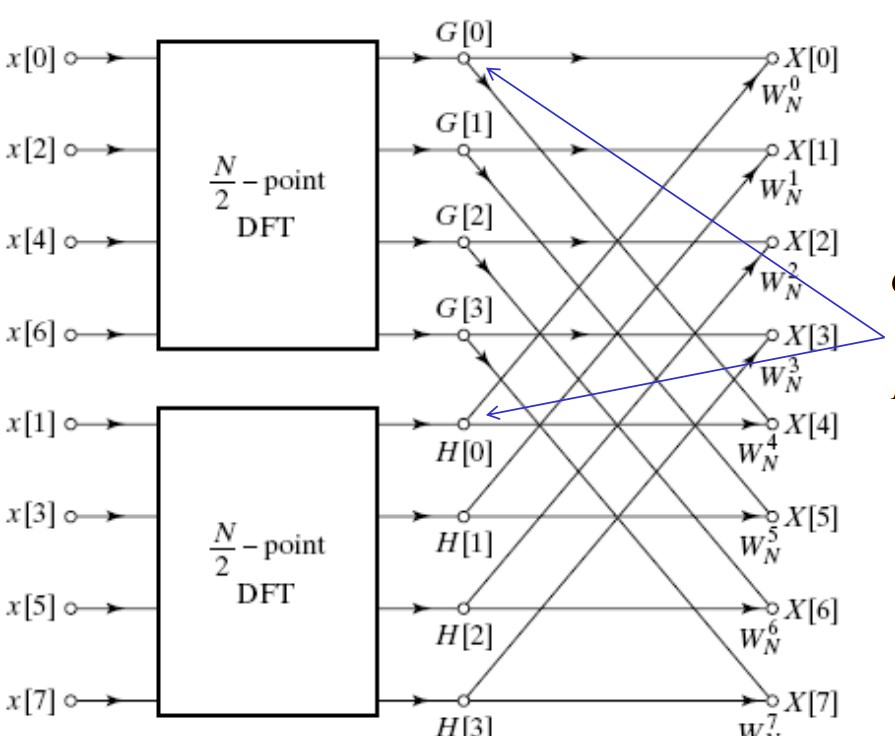
\includegraphics[width=6cm]{fft-dec-graph}
		\caption{graph representing the computation that are needed to be performed to compute the fast Fourier transform using the decimation in time algorithm for $N=8$ samples.}
	\end{SCfigure}
	
	
	By applying recursively this concept for sequences until we reach input signals of 2 samples each, the overall computational complexity of the \dft  drops from $\mathcal O(N^2)$ to $\mathcal O(N\log_2N)$.
	\begin{SCfigure}[2][bht]
		\centering 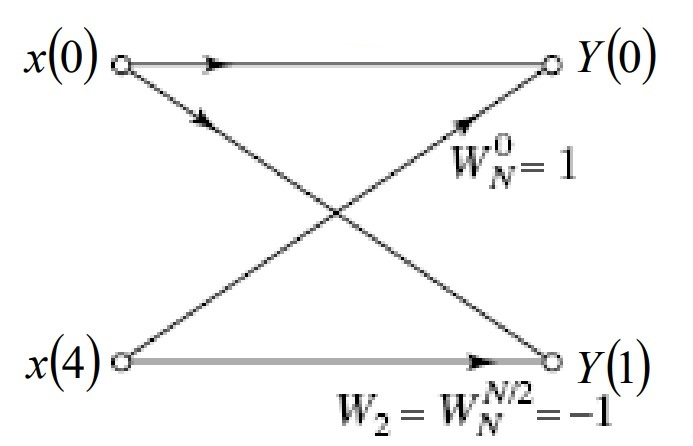
\includegraphics[width=4cm]{fft-dec-graph-bin}
		\caption{graph representation of the \fft using the decimation in time algorithm computed on 2 points.} \label{fig:dft:ditsing}
	\end{SCfigure}
	
	In the single stage (figure \ref{fig:dft:ditsing}) the transform become just a summation of the points we are considering, in fact
	\[ Y(0) = x(0) + x(1) \qquad \qquad \qquad Y(1) = x(0)-x(1) \]	
	Given the initial number $N$ of samples, then it means that we have to compute $2$ operation for each of the $N/2$ \textit{basic block} for the Fourier transform, and so the complexity presents a linear order. Laterly we need to \textit{join} the singularly computed block considering that the different twiddle factors are going each time to shift in the complex axis the spectrum inherited from the previous block; each stage also presents a linear order of complexity. The number of stages to be computed is equal to $\nu = \log_2N$ and so that's why the overall complexity of the algorithm is
	\[ \mathcal O\big(N\log_2 N \big) \]
	
	
	\begin{SCfigure}[2][bht]
		\centering 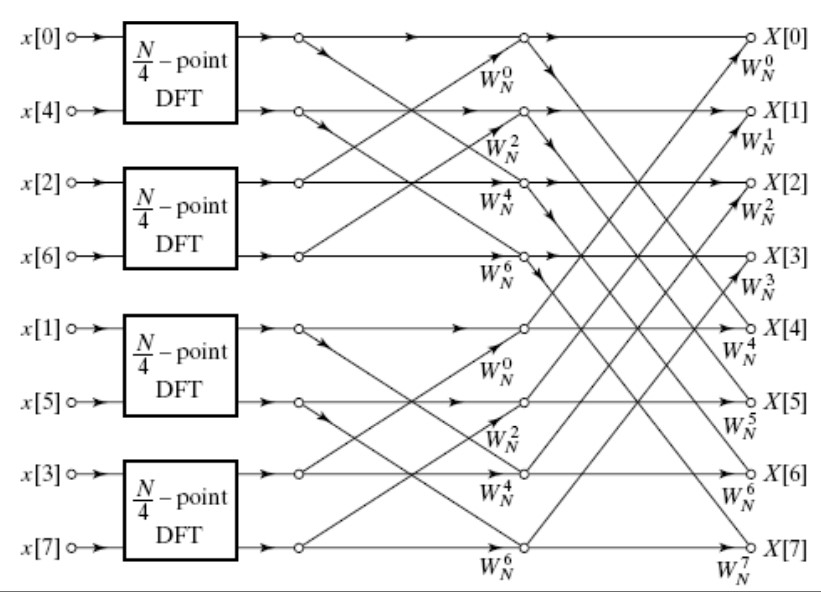
\includegraphics[width=7cm]{fft-dec-graph-comp}
		\caption{complete graph representing the computation to do with the decimation in time algorithm for $N=8$ samples. The transform of 2 value is shown in figure \ref{fig:dft:ditsing}.}
	\end{SCfigure}
	
	\paragraph{Modularity of the FFT algorithm} A point of force of this algorithm is it's recursion and modularity that allows to easily compute and \textit{see} different stages and tasks due to the \textit{butterfly structure}. Another strong point of implementation is that each operation permits to overwrite the spectrum on the same memory cell of the original signal. Also twiddle factors that need to be computed are equal for butterflies at each stage, and so they have to be computed one.
	
	In general the butterfly can be represented as in figure \ref{fig:dft:decstage} where the only thing that changes are the indexes $p,q$; to reduce the computation we can also see that 
	\[ W_N^{r + \frac{N}{2}} = W_N^r W_N^{\frac N 2}  = - W_N^r \]
	where $r$ depends on the stage we are considering.
	
	\begin{figure}[bht]
		\centering 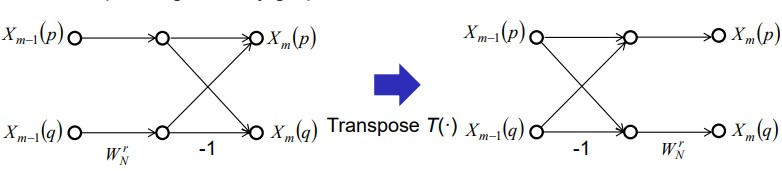
\includegraphics[width = 8cm]{fft-dec-stage}
		\caption{schematic representation of a generic stage of the decimation in frequency FFT algorithm.}
		\label{fig:dft:decstage}
	\end{figure}
	
	Another computational aspect that we might see is the use of memory; in fact samples are stored not in order for computation, however we can see that that the bits are inserted in \textbf{binary flip revered order} as in the example on table \ref{tab:dft:reversed}.
	\begin{SCtable}[2][bht]
		\centering
		\begin{tabular}{c c | c c}
			$x(0)$ & 000 & 000 & $X(0)$ \\
			$x(4)$ & 100 & 001 & $X(1)$ \\
			$x(2)$ & 010 & 010 & $X(2)$ \\
			$x(6)$ & 110 & 011 & $X(3)$ \\
			$x(1)$ & 001 & 100 & $X(4)$ \\
			$x(5)$ & 101 & 101 & $X(5)$ \\
			$x(3)$ & 011 & 110 & $X(6)$ \\
			$x(7)$ & 111 & 111 & $X(7)$ \\
		\end{tabular} \caption{example of binary revered order that's used in performing the the fast Fourier transform.} \label{tab:dft:reversed}
	\end{SCtable}
	
\subsection{Decimation in frequency FFT}
	This kind of FFT algorithm is an alternative to decimation in time one and in general it's complementary and it's based on the partition of the original signal in sub samples and so starting from the transform $X(k)$ we determine the partition in even and odd partition in the frequency:
	\[ X(k) \qquad \rightarrow \quad X_e(k ) = X(2k) \quad X_o(k) = X(2k+1) \]
	The concept of work is similar to the decimation in time and the algorithm presents a complexity of $\mathcal O(N\log_2N)$. This operation can be performed considering the \textbf{transpose property of the graph}: given a graph $\delta(N,\varepsilon)$ of $N$ edges and $\varepsilon$ edges, then it's transpose $\delta^t(N,\varepsilon')$ (where we reverse the edge direction, and so also input/output are reversed) the input-output relation of the graphs is the same. 
	
\section{Spectral estimation}
	The \de{spectral estimation} is an analyses of the signal that tends to provide information about the behaviour of the system.
	
	Considering that usually signals are not deterministic (but stochastic), this operation is usually hard to perform and handle; in general this operation is classified (figure \ref{fig:dft:estimation}) depending on the type of signal (deterministic or random) and it's stationarity.
	
	\begin{SCfigure}[1][bht]
		\centering 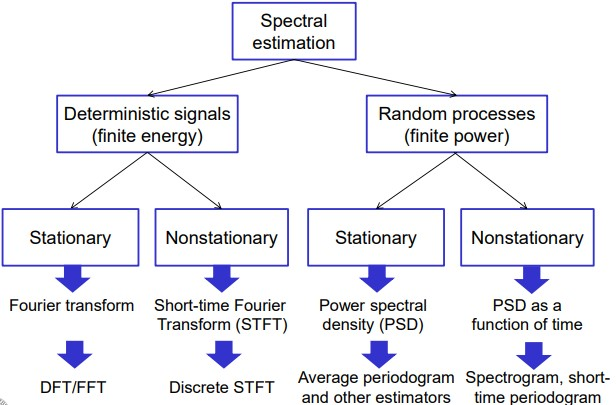
\includegraphics[width=7cm]{spectral-estimation}		
		\caption{classification of the spectral estimation} \label{fig:dft:estimation}
	\end{SCfigure}
	
	If a system is stationary the quality of estimation doesn't depend on the time on which we perform the estimation itself, while this isn't true for non-stationary signals on which we want to track all the changes of the signals.
	
	\paragraph{Deterministic stationary estimation} Focusing on a deterministic stationary signal $x_c(t)$, performing the spectral estimation is in theory easy because (with the Fourier transform) we can compute it's spectrum $X_c(\Omega)$. In practise however we cannot reach this exact value, but we get an approximation $\hat X_c(\Omega) \approx X_c(\Omega)$.
	
	\begin{figure}[bht]
		\centering
		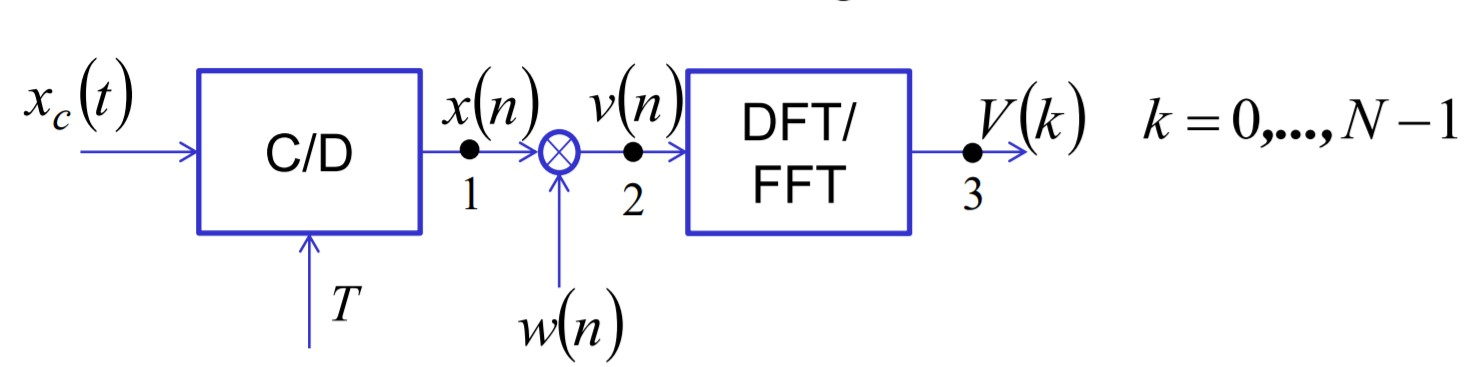
\includegraphics[width=8cm]{deterministic-estimation}
		\caption{step encountered while estimating a deterministic signal.}
		\label{fig:dft:deterministicestim}
	\end{figure}
	
	As we can see in figure \ref{fig:dft:deterministicestim} when dealing with a real world application of spectral estimation, the original signal $x_c(t)$ must be discretized in the time axis with a sampling period $T_s$ (and in this case we can consider an ideal component, but in reality just only this operation can introduce errors due to acquisition noises...); at this point the ideal Fourier transform of the input signal becomes
	\[ X(e^{j\omega}) = \frac 1{T_s} \sum_{k=-\infty}^{\infty} X_c \left( \frac \omega {T_s}+ \frac{2\pi k}{T_s} \right)  \]
	As we can see this discretization introduces to the original spectrum a scaling factor of $1/T_s$ and also introduces the spectral replicas at multiple frequencies of $2\pi/T_s$, and in  this case we neglect the quantization/acquisition noises.
	
	With the signal acquired the numerical tool that we can use to estimate the spectrum are the DFT/FFT algorithms that uses a finite number $N$ of samples (on which to compute the spectrum), and so the sequence $x(n)$ must be \textit{truncated} to such a number of samples: this operation is referred as \textbf{windowing}. This operation can be modelled as a multiplication of the initial sequence $x(n)$ with the function $w(n)$ defined as
	\[ w(n) = \begin{cases}
		1 \qquad& n=0,\dots,L-1 \\ 0 & \textrm{otherwise}
	\end{cases} \]

	At this point we can see that the DFT/FFT algorithm are applied on the sequence $v(n) = x(n)w(n)$ (on which we can see that $v(n) \neq 0$ for $n = 0,\dots, L-1$): by a spectral point of view this means that the estimated spectrum (considering the ideal Fourier transform) becomes
	\[ V(e^{j\omega}) = X(e^{j\omega}) * W(e^{j\omega}) = \frac 1{2\pi} \int_{-\pi}^\pi X(e^{j\theta}) W(e^{j(\omega-\theta)}) \, d\theta \neq X(e^{j\omega}) \]
	As a rule of thumb we see that the number of point $N$ on which we compute the \dft must be greater of equal to $L$, the number of \textit{windowed} samples (in reality $N$ can be less then $L$ if we don't have to go back in the time domain because the time aliasing won't be a problem, but we decrease also the \textit{resolution}).\\
	The final output $\hat X_c(\Omega) = V(k)$ also contains the problem of the spectral sampling.

	\paragraph{Effects of windowing on the spectral estimation of a sine wave} Considering the continuous time sinusoidal signal $x_c(t) = A \cos(\Omega_0t + \theta_0)$, it's spectrum (figure \ref{fig:dft:cosspec}) consists of two dirac pulses at frequencies $\pm\Omega_0$ having complex amplitude $\frac  A2 e^{-j\theta_0}$.
		
	\begin{SCfigure}[2][bht]
		\centering 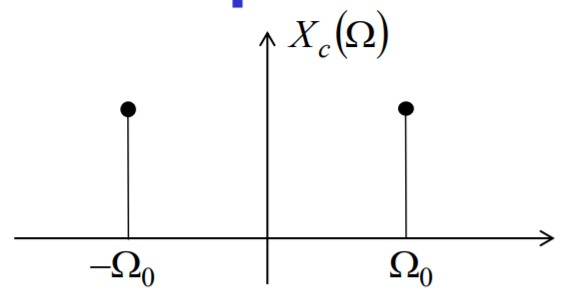
\includegraphics[width=5cm]{sin-spect}
		\caption{magnitude spectrum of the signal $A \cos(\Omega_0t+\theta_0)$.}
		\label{fig:dft:cosspec}
	\end{SCfigure}

	Assuming to sample the signal with a sampling period $T_s$ we determine the sequence $x(n) = A \cos(\omega_0n + \theta_0)$ (where $\omega_0 = \Omega_0 T_s$); considering on top of that the windowing the signal on which we can compute the DFT becomes
	\[ v(n) = x(n)w(n) = A w(n) \cos(\omega_0n+\theta_0) = \frac A 2 w(n) e^{j\theta_0} e^{j\omega_0n} +\frac A 2 w(n) e^{-j\theta_0} e^{-j\omega_0n} \]
	where we used the Euler relation. Applying the theoretical discrete-time Fourier transform we know that $\four{e^{j\omega_0n}} = \delta(\omega-\omega_0)$ and so the spectrum can be computed as
	\[ V\big(e^{j\omega}\big) = \frac A 2 e^{j\theta_0} W\big(e^{j(\omega-\omega_0)}\big) + \frac A 2 e^{-j\theta_0} W\big(e^{j(-\omega+\omega_0)}\big) \]
	At this point to determine the \textit{shape} of the estimated spectrum $V$ it's necessary to understand the distortion of the windows and so it's necessary to compute it's Fourier transform:
	\[ W\big(e^{j\omega}\big) = \sum_{n=-\infty}^{\infty} w(n) e^{-j\omega n} =  \sum_{n=0}^{L-1} e^{ -j\omega n} = \frac{1 - e^{-j\omega L}}{1-e^{-j\omega}} = e^{-j\omega \frac{L-1}{2}} \frac{\sin\left(\frac{\omega L}{2} \right)}{\sin \left( \frac \omega 2 \right)} \]
	where the series can be solved considering that $\sum e^{-j\omega n}$ is a geometrical progression. The special function $\sin\left(\frac{\omega L}{2}\right) / \sin\left(\frac \omega 2\right)$ is referred as Dirichlet-Kernel; characteristic of this function is that for $\omega= 0$, the magnitude of the spectrum is equal to $L$ and for each multiple of $2\pi/L$ it's null (figure \ref{fig:dft:dirich}).
	
	\begin{figure}[bht]
		\begin{subfigure}{0.48\linewidth}
			\centering 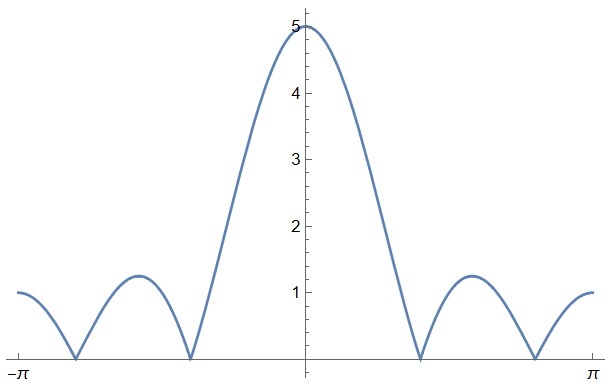
\includegraphics[width=5cm]{dirich-kernel} \caption{}
		\end{subfigure}
		\begin{subfigure}{0.48\linewidth}
			\centering 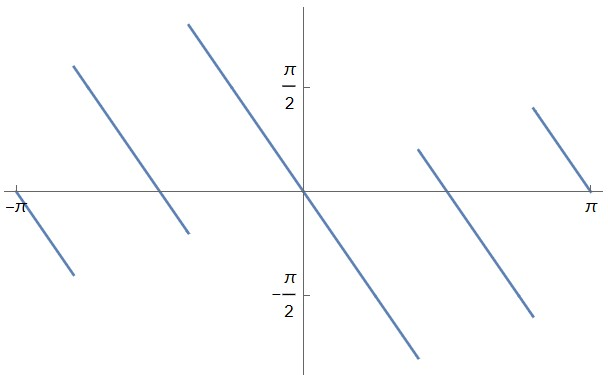
\includegraphics[width=5cm]{dirich-kernel-phase} \caption{}
		\end{subfigure}
		\caption{magnitude (a) and phase (b) of the Dirichlet-Kernel function.}
		\label{fig:dft:dirich}
	\end{figure}
	
	We refer to the \textit{central peek} as the main-lobe (and present a peek value equal to $L$ number of samples used for the windowing), while the other spectral \textit{bell-shapes} are the side-lobes whose maximum values is constantly decreasing for $\omega$ that increase. The parameter $\Delta_w = 4\pi /L$ represent the main-lobe width. The phase of this function is described as \textit{generalized linear phase}. \vspace{3mm}
	
	With that said, in theory the spectrum that we expect from the initial sinusoidal signal $x_c$ are two Dirac pulses, however in reality that spectrum $V(e^{j\omega})$ that we see (after the windowing due to the \textit{truncation} of the signal) is composed by two Dirichlet-Kernel function with main-lobes centred at the frequencies $\omega_0$ on which we expect the Dirac pulses (figure \ref{fig:dft:spectrdistorted}).
	
	\begin{SCfigure}[2][bht]
		\centering 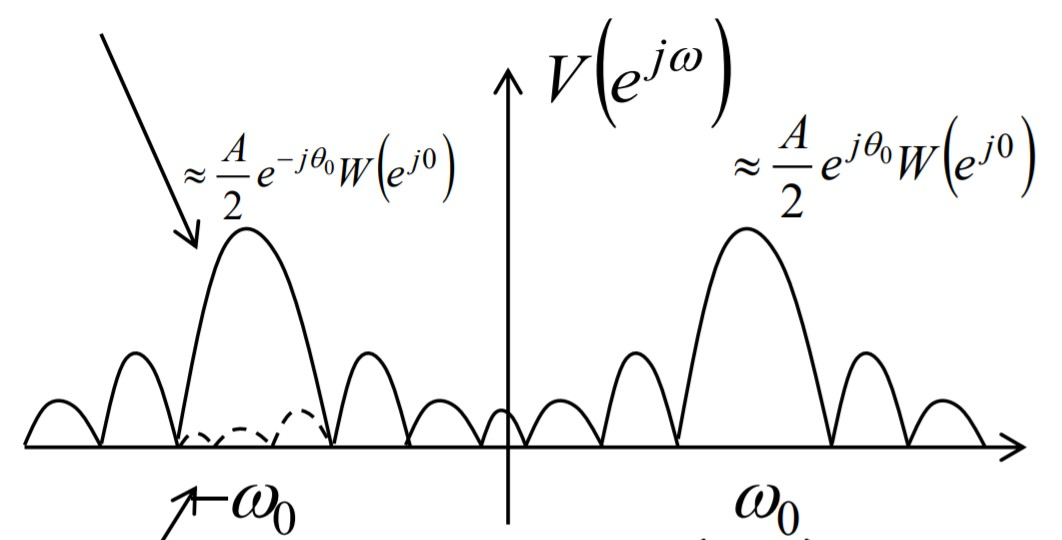
\includegraphics[width=6cm]{sin-modified}
		\caption{spectrum of the signal  $v(n)= x(n)w(n)$ that's distorted due to the windowing.}
		\label{fig:dft:spectrdistorted}
	\end{SCfigure}
	
	To decrease the main-lobe width $\Delta_w$ it's necessary to increase the number of sample $L$ considered on the window $w$ (in fact with $L\rightarrow \infty$ the Dirichlet-Kernel function tends to the Dirac pulse). In real world application we cannot get rid of the lobes of the Dirichlet-Kernel function (we cannot compute the DFT on sequence of infinite samples) and so the associated problems are 
	\begin{itemize}
		\item the \textbf{spectral leakage}: in theory the energy of the original sinusoidal signal is concentrated on the frequencies $\pm \omega_0$, however with the windowing  there's a sort of \textit{leak} that spread the energy over all the frequency axis;
		
		\item the \textbf{spectral infiltration} (related to the leakage) refers to the fact that the side-lobes of a Dirichlet-Kernel might interfere to the main-lobe of the other function (and vice-versa); it can be shown in fact that the ratio between the main-lobe and it's adjacent side-lobe is constant and weakly depend on the number of samples $L$;
		
		\item the \textbf{finite spectral resolution}: considering a signal $x_c(t) = A_1 \sin(\Omega_1t + \theta_1) + A_2 \sin(\Omega_2t + \theta_2)$, the ideal spectrum of the signal consist in Dirac pulses centred at frequencies $\pm \omega_1,\pm \omega_2$, however the estimated spectrum is in the form
		\[ V\big(e^{j\omega}\big) = \sum_i \frac{A_i}2 e^{\pm j\theta_i} W\Big( e^{j(\omega \mp \omega_i)} \Big) \]
		We can see that if the frequencies $\omega_1$ and $\omega_2$ are close together (mathematically $|\omega_1-\omega_2$ is \textit{small enough}) the main-lobes interferes and so the problem of the spectral leakage becomes very important and heavily changes the estimated spectrum. If the frequencies $\omega_1,\omega_2$ are \textit{far apart} this kind of problem might be neglected (figure \ref{fig:dft:spectralresolution}). Increasing the number $L$ the main-lobe width decrease and so we can qualitatively improve the spectral resolution. In order to not distinguish the two peeks (considering $A_1 = A_2$), as a qualitative definition, we must require that
		\[ |\omega_1-\omega_2| > \frac{\Delta_w}{2} \]
				
	\end{itemize}

	\begin{SCfigure}[2][bht]
		\centering 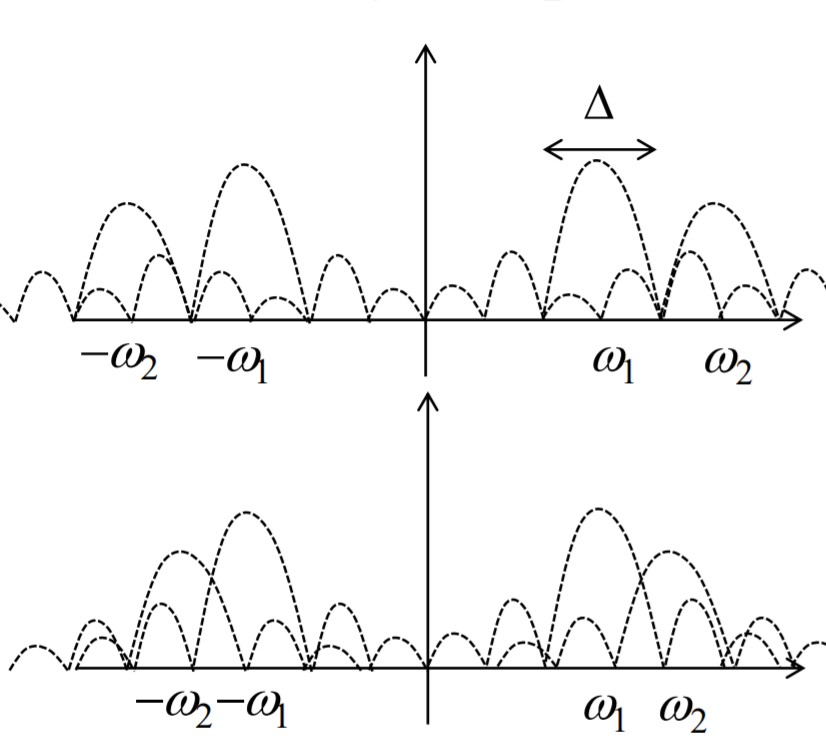
\includegraphics[width=6cm]{spectral-resolution}
		\caption{estimated spectrum of a signal $ A_1 \sin(\Omega_1t + \theta_1) + A_2 \sin(\Omega_2t + \theta_2)$ where the difference $\omega_1-\omega_2$ is negligible (upper) or not (lower) considering the problem of the spectral resolution.} \label{fig:dft:spectralresolution}
	\end{SCfigure}

	In general other window function $w(n)$ have been constructed in order to minimize the errors/problems associated to the spectral estimation (increasing the ratio between the main-lobe and the side-lobes and also decreasing the width $\delta_w$ given the same amount of samples $L$); this is achieved by not having rectangular shape but using smoother functions (table \ref{tab:dft:windowfunctions}, figure \ref{fig:dft:windowfunctions}).
	
	\begin{table} \centering
	\begin{tabular}{c|c|c}
		Windows & side/main-lobe ratio & main-lobe width $\Delta_w$\\ \hline
		rectangular & $-13db$ & $4\pi/L$ \\
		Bartlett (triangular) & $-25db$ & $8\pi/L$ \\
		Hanning & $-31db$ & $8\pi/L$ \\
		Hamming & $-41db$ & $8\pi/L$ \\
		Blackman & $-57db$ & $12\pi/L$ \\
	\end{tabular}
	\caption{list of possible windows with relative side to main-lobe radio (in decibels) and main-lobe width (depending on number of windowed samples $L$).}
	\label{tab:dft:windowfunctions}
	\end{table}
	\begin{figure}[bht]
		\centering 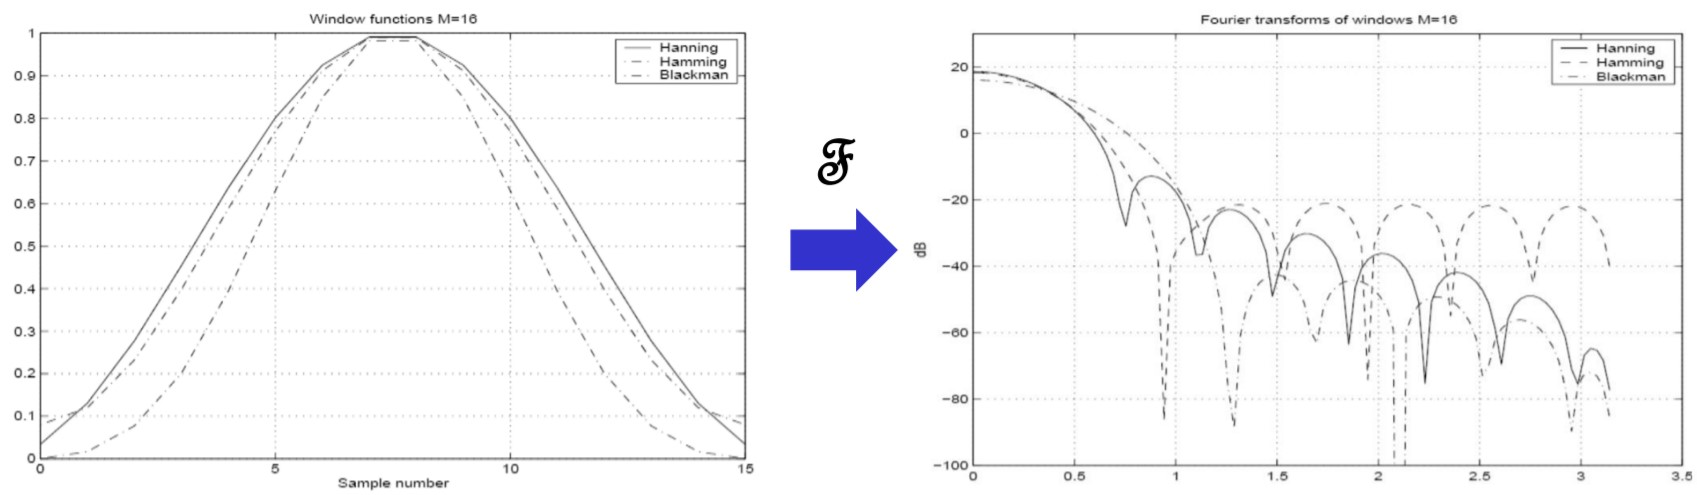
\includegraphics[width=\linewidth]{windowfunctions}
		\caption{windowing functions and relative Fourier transforms.}
		\label{fig:dft:windowfunctions}
	\end{figure}
		
	As we can see window functions with higher side to main-lobe attenuation  present main-lobe width that are higher (impacting so the resolution), but they also reduces the \textit{errors} due to the side-lobes. In particular Hanning, Hamming and Blackman are inside the so called \textbf{cosine class windows} of order $K$ that can generally expressed as
	\[ w(n) = \int_{k=0}^K a_k \cos\left( \frac{2\pi k}{L}n\right) \qquad n = 0,\dots, L-1 \]
	where the coefficients $a_k$ depends on the order $K$ chosen. In particular Hanning ($a_0 = \frac 1 2, a_1 = -\frac 1 2$) and Hamming ($a_0 = 0.54, a_1 = - 0.46$) windows are cosine class windows of order 1, while Blackman has order $2$. As we can see the main-lobe width relates to the order of the function following the relation
	\[ \Delta_w = \frac{4\pi}{L}\big(K+1\big) \]
	
	Fixing the samples $L$ of the transform going the rectangular to the Blackman windows the spectral resolution worsen while the spectral leakage improves (and so it's always a trade-off).	
	
	\paragraph{Frequency discretization} Until now we have computed the continuous spectrum $V(e^{j\omega})$ of the sampled signal, however by computing the \dft (or using \fft algorithms) what we get is just a discretization $V(k)$ (with $k =0,\dots,N-1$) on the frequency domain of the spectrum itself. In particular considering the initial case of the the sinusoidal function $x_c(t) = A \cos(\Omega_0 t + \theta_0)$ changing the number $N$ used for the computation of the DFT might heavily affect the read spectrum, and in particular we can have:
	\begin{itemize}
		\item a \textbf{coherent sampling} happens when one of the spectral samples lies exactly at the frequency $\omega_0$ while the other samples coincides with the zeros due to the window spectrum. In this case the spectrum is clear and the effect of leakage is negligible. This kind of operation can be performed in general only for periodic signals (because it's \textit{easy} to determine the number of samples $N$ that minimize the leakage) due to the fact that the ideal spectrum is composed by a sequence of Dirac pulses;
		\item a \textbf{non-coherent sampling} happens when the peak lies between the two largest spectral samples; in this case we have uncertainty both in the magnitude and in the frequency of the peak. The effect of leakage is evident;
		\item improving the number of samples $N$ on a non-coherent sampling increases the number of spectral samples and so the error in estimating the magnitude and relative frequency of the peak decreases (but the effect of leakage doesn't decrease). 
	\end{itemize}
	
	\begin{figure}[bht]
		\begin{subfigure}{0.32\linewidth}
			\centering 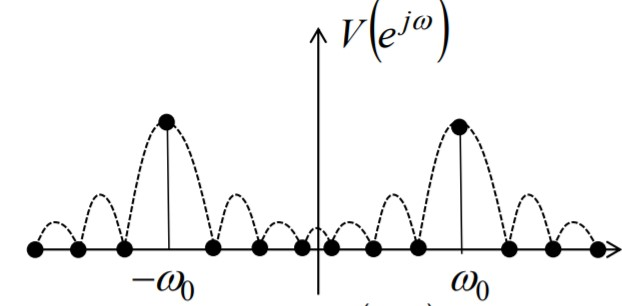
\includegraphics[width=0.9\linewidth]{sampling-1} \caption{}
		\end{subfigure}
		\begin{subfigure}{0.32\linewidth}
			\centering 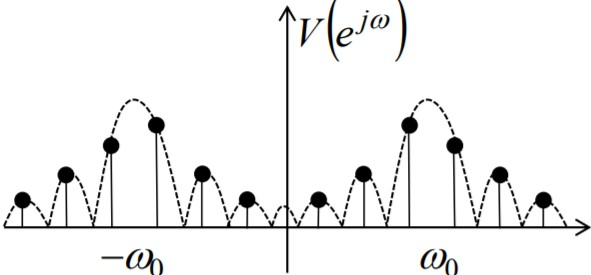
\includegraphics[width=0.9\linewidth]{sampling-2} \caption{}
		\end{subfigure}
		\begin{subfigure}{0.32\linewidth}
			\centering 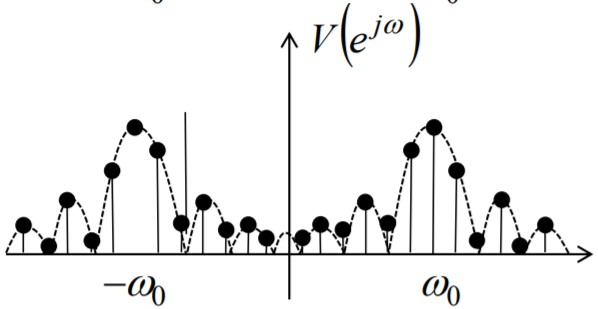
\includegraphics[width=0.9\linewidth]{sampling-3} \caption{}
		\end{subfigure}
		\caption{coherent sampling (a), non-coherent sampling (b) and non-coherent sampling with higher number of samples $N$ (c).}
		\label{fig:dft:samplingvariation}
	\end{figure}
	
	\paragraph{Non stationary deterministic signals} A simple example of non stationary signal is the \textbf{chirp} one defined as a sinusoidal function whose frequency changes linearly over time, and so of the form
	\[ x_c(t) = \cos\big(\Omega(t) t\big)  \qquad \textrm{where } \Omega(t) = \Omega_0t \]
	In this case evaluating the function at the time $t_0$ we expect a DFT having a Dirac pulse centred at frequency $\Omega(t_0)$, while if we evaluate the signal at time $t_1$ we expect a pulse at another frequency $\Omega(t_1)$. In the real world we cannot have this kind of spectrum because we have to compute the transform over a window of the real signal (whose frequency is changing over time); in particular the read spectrum is a sort of \textit{smoothed average} of the peaks in the transform in the range whose samples are extracted. To avoid this problem we can try to reduce the window in time $\Delta t$ (time from the first to last sample) but this impact in the number of samples $L$ recorded (decreasing the frequency resolution). In general
	\begin{align*}
		\textrm{long window} \qquad &\Rightarrow \quad \textrm{high frequency resolution, poor time resolution} \\
		\textrm{short window} \qquad &\Rightarrow \quad \textrm{low frequency resolution, good time resolution}
	\end{align*}
	
	Considering in general that we expect two peaks at frequencies $\Omega_1,\Omega_2$, than the related difference of normalized frequency $\Delta \omega = \Delta \Omega \, T_s$ must be at least equal to half of the main-lobe width, and so in the case of the rectangular window we can see that
	\[ \Delta \omega > \frac{\Delta_w}{2} = \frac{4\pi}{2L} \qquad \Rightarrow \quad \Delta_f \underbrace{L T_s}_{=\Delta t} > 1   \]
	This expression gives the lower bound between time analyses and frequency resolution (where $\Delta_f$ is the frequency difference between the components in the signal).
	
\subsection{Short time Fourier transform}
	The \de{short time Fourier transform}, also known as discrete-time time-varying Fourier transform is a operation that performs DFTs over $L$ samples by \textit{shifting} each time by $R$ samples; ideally we have a \textit{localised} Fourier transforms (and so with a short window we can improve the time resolution) that are spread over all the sample axis. In general we consider $R\leq L$ in order to not lose information (in fact if $R>L$ a number of $R-L$ samples will be lost because they won't be used in the computation of the DFT), while as for the previous cases usually $L\leq N$ in order to have a better read-out of the spectrum.
	
\subsection{Estimation of the power spectral density}
	As seen on page \pageref{eq:prob:psd}, the power spectral density is the Fourier transform of the auto-correlation of a wide sense stationary random process. In real world application it's necessary to estimate this spectrum $\hat \Phi(e^{j\omega})$ that's in general computationally heavier than a single Fourier transform (because the auto-correlation contains a summation in it's definition).
	
	Given a continuous signal $x_c(t)$ sampled with period $T_s$ to determine the sequence $x(n)$ that's then windowed by the window $w(n)$, the estimation of the power spectral density can be achieved in two ways:
	\begin{itemize}
		\item by firstly computing the autocorrelation of the windowed signal that's lately transformed. Starting from the definition of the discrete-time autocorrelation (eq. \ref{eq:four:autocorrelation}, pg. \pageref{eq:four:autocorrelation}) considering as window function the rectangular one with $L$ samples, then the autocorrelation of the sequence $v(n) = x(n)w(n)$ can be computed as
		\begin{equation} \label{eq:dft:windowedauto}
			\hat \phi_v(n) = \frac 1 L \sum_{l=0}^{L-|n|-1} x(l) x(n+l) \qquad \textrm{with } n = 0,\dots,L-1
		\end{equation}
		At this point we can compute the estimation of the power spectral density $\hat \Phi_v(e^{j\omega})$ by computing the Fourier transform $\four{\phi_v(n)}$ of the computed autocorrelation over $L$ samples;
		
		\item by inverting the steps we can firstly compute a discretized sequence of the spectrum $V(k) = \four{v(n)}$ that's then passed through a \textit{power spectral density estimator} that computes $\hat \Phi_v(e^{j\omega})$ (or in practise it's discretization over the frequency axis). This operation is usually peformed by the \textbf{periodogram} that will be described later.
	\end{itemize}
	
	\paragraph{Estimator} An \de{estimator} is any function that, given a random sampled from the population, infers a parameter of the population that's taken from. An example of estimator is the one that, given $M$ person of a cities, tends to compute the average age of the city. The estimator $E\{\cdot\}$ is in this case examples the mean value of the samples that's
	\[ E\{x\} = \frac 1 M \sum_{i=1}^M x_i \]
	where $E\{x\}$ is the estimated age average of the population $x$ and where $x_i$ are the age of the sampled person. \vspace{3mm}
	
	The goal now is to fined a function $g$ that allows to better estimate the power spectral density of a given sequence that's already been transformed (and so it's in the frequency domain). Consider $\boldsymbol x$ as the random vector of all the possible inputs, then the estimated power spectral density $\hat \theta = g(\boldsymbol x)$ becomes a random process that's for each input $\boldsymbol x$, $\theta$ is the realization of the random process.\\
	Consider that $\hat \theta$ is a random process, than it's characterized by a probability density function that can be used to determine the expected value $E\{\hat \theta\}$ and it's variance $\textrm{Var}\{\hat \theta\}$ that, for an ideal estimator, should be $E\{\hat \theta\} = \theta$ and $V\{\hat \theta\} = 0$. In general we defined
	\[ E \{\hat \theta\} = \begin{cases}
		\theta \qquad & \textrm{unbiased estimator} \\
		\theta + c\qquad & \textrm{biased estimator}
	\end{cases}\]
	\[ V\{ \hat \theta \} \xrightarrow{M\rightarrow \infty} \begin{cases}
		=0 \qquad & \textrm{consistent estimator} \\
		\neq 0 & \textrm{inconsistent estimator}
	\end{cases} \]
	In general the problem of the bias of the estimator can be handled, while the same cannot be said for the consistency of the variance. 
	
	\paragraph{Characteristic of the estimation of the autocorrelation} Given the windowed signal $v(n) = x(n) w(n)$, the autocorrelation of each sample can be computed as shown in equation \ref{eq:dft:windowedauto}. Given $X(\cdot)$ the associated random process, the estimation of the random process can be computed as
	\begin{align*}
		E\left\{\hat \Phi_V(n)\right\} & = E \left\{ \frac 1 L  \sum_{l=0}^{L-|n|-1} X(l) X(n+l) \right\} = \frac 1 L \sum_{l=0}^{L-|n|-1} \phi_x(n) \\
		& = \frac{L-|n|}{L} \phi_x(n)
 	\end{align*} 
	This means that this kind of estimation in biased with a variant level depending from the window length $L$ and the \textit{position} $n$ of the sample. In general the performance are good for $n\ll L$. Similarly we can show that this estimation is non consistent, in fact it can be shown that
	\[ V\left\{ \hat \Phi_V \right\} = E\left\{ \hat \Phi_v^2(n) \right\} - E\left\{ \hat \Phi_v(n) \right\}^2 = \alpha \phi_x^2(n) \]
	
	\paragraph{Ideal periodogram} The \de{periodogram} is a particular power spectral density estimator defined as
	\begin{equation}
		\hat \Phi_V(e^{j\omega}) = \frac{|V(e^{j\omega})|^2}{L} \qquad V(e^{j\omega}) = \four{v(n)}
	\end{equation}
	By extending the definition of the spectrum $V(e^{j\omega})$ computed on the windowed signal we can similarly rewrite this estimator as
	\begin{align*}
		\hat \Phi_V(e^{j\omega}) & = \frac 1 L \Big( \sum_{n=-\infty}^\infty x(n) w(n) e^{-j\omega n} \Big)( \sum_{m=-\infty}^\infty x(n) w(n) e^{-j\omega m} \Big)^* \\ & = \frac 1 L \Big( \sum_{n=-\infty}^\infty x(n) w(n) e^{-j\omega n} \Big)( \sum_{m=-\infty}^\infty x^*(n) w(n) e^{j\omega m} \Big) \\ 
		& = \frac 1 L \sum_{n=-\infty}^\infty\sum_{m=-\infty}^\infty x(n) x^*(m) w(n) w(m) e^{-j\omega(n-m)}
	\end{align*}

	With this definition stated we can compute the expectation of the estimator as
	\begin{align*}
		E\left\{ \hat \Phi_V \right\} & = \frac 1 L \sum_{n=-\infty}^\infty\sum_{m=-\infty}^\infty \overbrace{E\left\{x(n) x^*(m)\right\}}^{= \phi_x(m) \textrm{: autocorrelation}} w(n) w(m) e^{-j\omega(n-m)} \\
		\xrightarrow{n-m=k} \quad & = \frac 1 L \sum_{m=-\infty}^\infty \sum_{k=-\infty}^\infty \phi_x(k) w(m) w(m+k) e^{-j\omega k} \\
		& = \frac 1 L \underbrace{\sum_{k=-\infty}^\infty \phi_x(k) e^{-j\omega k}} \underbrace{\sum_{m=-\infty}^\infty w(m) w(m+k)} 
	\end{align*}
	In this expression the first underlined term represent the power spectral density value that has to be estimated, while the second one is the autocorrelation $\mathcal E_w(k)$ of the window function that represent a sort of \textit{weight} in the evaluation of the expectation. Applying now to this result the Parseval's theorem (eq. \ref{eq:four:parserval}, pg. \pageref{eq:four:parserval}) the expectation can be computed as
	\begin{align*}
		E\left\{ \hat \Phi_V \right\} & = \frac 1 {2\pi L} \int_{-\pi}^\pi \phi_x ()e^{j\theta}) \mathcal C_w(e^{j(\omega-\theta)}) \, d\theta = \frac 1 L \phi_x (e^{j\omega}) * |W(e^{j\omega})|^2
	\end{align*}
	This means that this estimator is biased by a factor $*\frac1 L |W(e^{j\omega})|^2$ depending so on the chosen window.
	
	
	
	
	
	
	
	
	
	
	
	
	
	
	
	
	
	
	
	
	
	